% ---------------------------------------------------------------------------
% ---------------------------------------------------------------------------
% Junção de templates encontrados no Overleaf
% facilitando a vida do aluno de pós da UFABC
% Modelo LaTex para preparação do documento final de Dissertação de Mestrado
% ninguém do programa de pós da informação validou se presta
% ---------------------------------------------------------------------------
% ---------------------------------------------------------------------------

\documentclass[
	% -- opções da classe memoir --
	12pt,					% tamanho da fonte
	openright,				% capítulos começam em pág ímpar (insere página vazia caso preciso)
	twoside,					% para impressão em verso e anverso. Oposto a oneside
	a4paper,					% tamanho do papel. 
	% -- opções da classe abntex2 --
	%chapter=TITLE,			% títulos de capítulos convertidos em letras maiúsculas
	%section=TITLE,			% títulos de seções convertidos em letras maiúsculas
	%subsection=TITLE,		% títulos de subseções convertidos em letras maiúsculas
	%subsubsection=TITLE,	% títulos de subsubseções convertidos em letras maiúsculas
	% -- opções do pacote babel --
	english,					% idioma adicional para hifenização
	%french,					% idioma adicional para hifenização
	%spanish,				% idioma adicional para hifenização
	brazil					% o último idioma é o principal do documento
	]{abntex2}

% ---------------------
% Pacotes OBRIGATÓRIOS
% ---------------------
\usepackage{lmodern}				% Usa a fonte Latin Modern			
\usepackage[T1]{fontenc}			% Selecao de codigos de fonte.
\usepackage[utf8]{inputenc}		% Codificacao do documento (conversão automática dos acentos)
\usepackage{lastpage}			% Usado pela Ficha catalográfica
\usepackage{indentfirst}			% Indenta o primeiro parágrafo de cada seção.
\usepackage{color}				% Controle das cores
\usepackage{graphicx,graphicx}	% Inclusão de gráficos
\usepackage{epsfig,subfig}		% Inclusão de figuras
\usepackage{microtype} 			% Melhorias de justificação
\usepackage{float}
% ---------------------
		
% ---------------------
% Pacotes ADICIONAIS
% ---------------------
\usepackage{lipsum}						% Geração de dummy text
\usepackage{amsmath,amssymb,mathrsfs, upgreek}	% Comandos matemáticos avançados 
\usepackage{setspace}  					% Para permitir espaçamento simples, 1 1/2 e duplo
\usepackage{verbatim}					% Para poder usar o ambiente "comment"
\usepackage{tabularx} 					% Para poder ter tabelas com colunas de largura auto-ajustável
\usepackage{afterpage} 					% Para executar um comando depois do fim da página corrente
\usepackage{url} 						% Para formatar URLs (endereços da Web)
% ---------------------

% ---------------------
% Pacotes de CITAÇÕES
% ---------------------
\usepackage[brazilian,hyperpageref]{backref}	% Paginas com as citações na bibl
\usepackage[alf]{abntex2cite}				% Citações padrão ABNT (alfa)
%\usepackage[num]{abntex2cite}				% Citações padrão ABNT (numericas)
% ---------------------

\setcounter{MaxMatrixCols}{20}

% Configurações de CITAÇÕES para abntex2
% --- 
% CONFIGURAÇÕES DE PACOTES
% --- 

% ---
% Configurações do pacote backref
% Usado sem a opção hyperpageref de backref
\renewcommand{\backrefpagesname}{Citado na(s) página(s):~}
% Texto padrão antes do número das páginas
\renewcommand{\backref}{}
% Define os textos da citação
\renewcommand*{\backrefalt}[4]{
	\ifcase #1 %
		Nenhuma citação no texto.%
	\or
		Citado na página #2.%
	\else
		Citado #1 vezes nas páginas #2.%
	\fi}%
% ---

% Inclusão de dados para CAPA e FOLHA DE ROSTO (título, autor, orientador, etc.)
% ---
% Informações de dados para CAPA e FOLHA DE ROSTO
% ---
\titulo{Este é o Título da Dissertação}
\autor{Autor da Dissertação}
\local{Santo André - SP}
\data{Xxxx de 20XX}
\orientador{Fulano Nome do Orientador}
\coorientador{Fulano Nome do Coorientador}
\instituicao{%
  Universidade Federal do ABC -- UFABC
  \par
  Centro de Engenharia, Modelagem e Ciências Sociais Aplicadas 
  \par
  Programa de Pós-Graduação em Engenharia da Informação}
\tipotrabalho{Dissertação (Mestrado)}
% O preambulo deve conter o tipo do trabalho, o objetivo,
% o nome da instituição e a área de concentração
\preambulo{\textbf{Dissertação de Mestrado} apresentada ao Programa de Pós-Graduação em Engenharia da Informação (área de concentração: Sistemas Inteligentes), como parte dos requisitos necessários para a obtenção do Título de Mestre em Engenharia da Informação.}
% ---

% Inclui Configurações de aparência do PDF Final
%  Configurações de aparência do PDF final
% NÃO ALTERAR!!!

% alterando o aspecto da cor azul
\definecolor{blue}{RGB}{41,5,195}

% informações do PDF
\makeatletter
\hypersetup{
     	%pagebackref=true,
		pdftitle={\@title}, 
		pdfauthor={\@author},
    		pdfsubject={\imprimirpreambulo},
	    pdfcreator={LaTeX with abnTeX2},
		pdfkeywords={abnt}{latex}{abntex}{abntex2}{trabalho acadêmico}, 
		colorlinks=true,       		% false: boxed links; true: colored links
    		linkcolor=blue,          	% color of internal links
    		citecolor=blue,        		% color of links to bibliography
    		filecolor=magenta,      		% color of file links
		urlcolor=blue,
		bookmarksdepth=4
} 
\makeatother
% --- 

% O tamanho da identação do parágrafo é dado por:
\setlength{\parindent}{1.3cm}

% Controle do espaçamento entre um parágrafo e outro:
\setlength{\parskip}{0.2cm}  % tente também \onelineskip

% ---------------------
% Compila o indice
% ---------------------
\makeindex
% ---------------------

%%%%%%%%%%%%%%%%%%%%%%%%%%%
%%  INICIO DO DOCUMENTO  %%
%%%%%%%%%%%%%%%%%%%%%%%%%%%
\begin{document}

% Retira espaço extra obsoleto entre as frases.
\frenchspacing

% ----------------------------------------------------------
% ELEMENTOS PRÉ-TEXTUAIS (Capa, Resumo, Abstract, etc.)
% ----------------------------------------------------------
\pretextual

% Capa
% ---
% Impressão da Capa
% ---
  \begin{capa}%
    \begin{figure}[h!]%
        \centering%
        
\includegraphics[scale=1.2]{figs/logo.png}%
      \end{figure}%
    \center
	\ABNTEXchapterfont\large{Universidade Federal do ABC \\ Centro de Engenharia, Modelagem e Ciências Sociais Aplicadas}
	%\vspace{1.5cm}

    \vfill
    \ABNTEXchapterfont\bfseries\LARGE\imprimirtitulo
    \vfill

	%\vfill
	\ABNTEXchapterfont\large\imprimirautor
	\vfill
%

	
    \large\imprimirlocal, \large\imprimirdata

    \vspace*{1cm}
  \end{capa}
% ---

% Folha de rosto (o * indica que haverá a ficha bibliográfica)
\imprimirfolhaderosto*

% Imprimir Ficha Catalografica
% ---
% Ficha Catalográfica
% ---
% Isto é um exemplo de Ficha Catalográfica, ou ``Dados internacionais de
% catalogação-na-publicação''. Você pode utilizar este modelo como referência. 
% Porém, talvez a biblioteca lhe fornece um PDF
% com a ficha catalográfica definitiva após a defesa do trabalho. Quando estiver
% com o documento, salve-o como PDF no diretório do seu projeto e substitua todo
% o conteúdo de implementação deste arquivo pelo comando abaixo:
%
% \begin{fichacatalografica}
%     \includepdf{fig_ficha_catalografica.pdf}
% \end{fichacatalografica}
\begin{fichacatalografica}
	\vspace*{\fill}					% Posição vertical
	\hrule							% Linha horizontal
	\begin{center}					% Minipage Centralizado
	\begin{minipage}[c]{12.5cm}		% Largura
	
	\imprimirautor
	
	\hspace{0.5cm} \imprimirtitulo  / \imprimirautor. --
	\imprimirlocal, \imprimirdata-
	
	\hspace{0.5cm} \pageref{LastPage} p. : il. (algumas color.) ; 30 cm.\\
	
	\hspace{0.5cm} \imprimirorientadorRotulo~\imprimirorientador\\
	
	\hspace{0.5cm}
	\parbox[t]{\textwidth}{\imprimirtipotrabalho~--~\imprimirinstituicao,
	\imprimirdata.}\\
	
	\hspace{0.5cm}
		1. Palavra-chave1.
		2. Palavra-chave2.
		I. Orientador.
		II. Universidade xxx.
		III. Faculdade de xxx.
		IV. Título\\ 			
	
	\hspace{8.75cm} CDU 02:141:005.7\\
	
	\end{minipage}
	\end{center}
	\hrule
\end{fichacatalografica}
% ---

% Inserir Folha de Aprovação
% ---
% Assinaturas
% ---
% Isto é um exemplo de Folha de aprovação, elemento obrigatório da NBR
% 14724/2011 (seção 4.2.1.3). Você pode utilizar este modelo até a aprovação
% do trabalho. Após isso, substitua todo o conteúdo deste arquivo por uma
% imagem da página assinada pela banca com o comando abaixo:
%
% \includepdf{folhadeaprovacao_final.pdf}
%
\begin{folhadeaprovacao}

  \begin{center}
    {\ABNTEXchapterfont\large\imprimirautor}

    \vspace*{\fill}\vspace*{\fill}
    \begin{center}
      \ABNTEXchapterfont\bfseries\Large\imprimirtitulo
    \end{center}
    \vspace*{\fill}
    
    \hspace{.45\textwidth}
    \begin{minipage}{.5\textwidth}
        \imprimirpreambulo
    \end{minipage}%
    \vspace*{\fill}
   \end{center}
        
 % Isso na versao final do trabalho!!!       
   Trabalho aprovado. \imprimirlocal, 01 de janeiro de 2014:

   \assinatura{\textbf{\imprimirorientador} \\ Orientador} 
   \assinatura{\textbf{\imprimircoorientador} \\ Co-Orientador} 
   \assinatura{\textbf{Professor} \\ Convidado 1}
   \assinatura{\textbf{Professor} \\ Convidado 2}
   \assinatura{\textbf{Professor} \\ Convidado 3}
      
   \begin{center}
    \vspace*{0.5cm}
    {\large\imprimirlocal}
    \par
    {\large\imprimirdata}
    \vspace*{1cm}
  \end{center}
  
\end{folhadeaprovacao}
% ---

% Dedicatória
% ---
% Dedicatória
% ---
\begin{dedicatoria}
   \vspace*{\fill}
   \centering
   \noindent
   \textit{ Aos verme que roeu as frias carnes de meu cadáver.} \vspace*{\fill}
\end{dedicatoria}
% ---

% Agradecimentos
% ---
% Agradecimentos
% ---
\begin{agradecimentos}



Agradeço a Xuxa, meus pais, cachorro, gato e papagaio, por ...

Agradeço ao meu orientador, XXXXXXXXX, por todos os conselhos, pela paciência e ajuda nesse período.

Aos meus amigos ...

Aos professores ...

À XXXXXX pelo apoio financeiro para realização deste trabalho de pesquisa.

\end{agradecimentos}
%% ---

% Epígrafe
% ---
% Epígrafe
% ---
\begin{epigrafe}
    \vspace*{\fill}
	\begin{flushright}
		\textit{``Não sei o que, \\
		          não sei o que,\\
                  não sei o que lá.''\\
		          (Autor Desconhecido)}
	\end{flushright}
\end{epigrafe}
% ---

% Resumo e Abstract
% ---
% RESUMOS
% ---

% RESUMO em português
\setlength{\absparsep}{18pt} % ajusta o espaçamento dos parágrafos do resumo
\begin{resumo}
 Segundo a ABNT, o resumo deve ressaltar o
 objetivo, o método, os resultados e as conclusões do documento. A ordem e a extensão
 destes itens dependem do tipo de resumo (informativo ou indicativo) e do
 tratamento que cada item recebe no documento original. O resumo deve ser
 precedido da referência do documento, com exceção do resumo inserido no
 próprio documento. Umas 10 linhas (\ldots) As palavras-chave devem figurar logo abaixo do
 resumo, antecedidas da expressão Palavras-chave:, separadas entre si por
 ponto e finalizadas também por ponto.

 \textbf{Palavras-chave}: latex. abntex. editoração de texto.
\end{resumo}

% ABSTRACT in english
\begin{resumo}[Abstract]
 \begin{otherlanguage*}{english}
   This is the english abstract.

   \vspace{\onelineskip}
 
   \noindent 
   \textbf{Keywords}: latex. abntex. text editoration.
 \end{otherlanguage*}
\end{resumo}

% Lista de ilustrações
\pdfbookmark[0]{\listfigurename}{lof}
\listoffigures*
\cleardoublepage

% Lista de tabelas
\pdfbookmark[0]{\listtablename}{lot}
\listoftables*
\cleardoublepage

% Lista de abreviaturas e siglas
\begin{siglas}
  \item[ABNT] Associação Brasileira de Normas Técnicas
  \item[abnTeX] Normas para TeX
  \item[MEF] Métodos de Elementos Finitos
\end{siglas}

% Lista de símbolos
\begin{simbolos}
  \item[$ \epsilon $] Deformação axial
  \item[$ \gamma $] Deformação angular
  \item[$ E $] Módulo de Young
  \item[$ G $] Módulo de Cisalhamento
  \item[$ \nu $] Coeficiente de Poisson 
  \item[$ \pmb{u}_{e} $]
  \item[$ \pmb{A} $] Matriz de coeficientes de deslocamentos dos nós
  \item[$ \pmb{D}_{e} $] Matriz de elasticidade
  \item[$ \epsilon_{e} $] Vetor de deformações
  \item[$ \pmb{B}_{e} $] Matriz de tensão-deformação
  \item[$ \pmb{K}_{e} $] Matriz de rigidez do elemento da estrutura
  \item[$ \pmb{K} $] Matriz de rigidez global da estrutura
  \item[$ \pmb{M} $] Matriz de massa da estrutura
   
  
\end{simbolos}

% Inserir o SUMÁRIO
\pdfbookmark[0]{\contentsname}{toc}
\tableofcontents*
\cleardoublepage

% ----------------------------------------------------------
% ELEMENTOS TEXTUAIS (Capítulos)
% ----------------------------------------------------------
\textual
% Elementos textuais com numeração arábica
\pagenumbering{arabic}
% Reinicia a contagem do número de páginas
\setcounter{page}{1}

% Inclui cada capitulo da Dissertação

\chapter{Introdução}\label{cap:introducao}

\section{Considerações Iniciais}
Após um terremoto, para aumentar as chances de sobrevivência das vitimas,
é fundamental prestar assistência médica nas primeiras 24 horas \cite{schultz1996medical}.
A dificuldade de realizar busca em meio a escombros, a baixa acessibilidade terrestre devido a danos na malha rodoviárias e o número limitado de equipes de busca são fatores que influenciam no andamento de uma missão de salvamento.
Para auxiliar as missões de resgate, robôs estão sendo cada vez mais empregados. Entretanto, um dos obstáculos a serem superados está em como levar esses dispositivos até sua área de atuação. 

Uma maneira promissora é o transporte aéreo até as regiões de interesse seguido do envio por paraquedas até o solo. 
O salto de paraquedas pode ser divido em três fases: o salto do avião, a abertura do paraquedas e a aterrissagem ao solo.
Este último se mostra o mais complexo devido às acelerações de impacto, que podem danificar os componentes frágeis de um robô durante um aterrissagem \cite{tsujita2017drop}.
Breves estudos mostraram a redução de impacto ao solo quando se utilizam materiais acolchoados \cite{tsujita2017drop} \cite{tsujita2017analysis}.
Este trabalho tem como objetivo dar continuidade a esses trabalhos, medindo a eficiência de tipos distintos de materiais acolchoados, na construção de um simulador de testes de queda, além da identificação de parâmetros de amortecimento de \textit{Rayleigh}.

Desastres naturais são eventos geológicos ou atmosféricos que possuem grande impacto econômico e social. Pode-se citar como exemplo: furacões, terremotos, tufões, tsunamis, deslizamentos, erupções vulcânicas e inundações\cite{naturaldisasters}.
Além do alto número de mortes e feridos, existem os danos às construções como escolas, fábricas, hospitais, na infraestrutura e produção rural\cite{benson1997economic}.
Dentre os maiores desastres naturais que ocorreram na última década, tem-se em 2010, o terremoto de magnitude 7.0 que atingiu o Haiti, causando cerca de 230.000 mortes, 300.000 feridos e um prejuízo avaliado em cerca de 8 bilhões de dólares\cite{haiti2010}.
No ano seguinte, em 2011, a região leste do Japão sofreu com um terremoto de magnitude 9.1 e o consequente tsunami. O incidente levou o falecimento de cerca de 16.000 pessoas, com um prejuízo avaliado em 199 bilhões de dólares \cite{tohoku2011}.
O mesmo país sofreu, em 2019, com o tufão de categoria 5, \textit{Hagibis}, que causou deslisamentos e inundações, levando a um prejuízo estimado em 10 bilhões de dólares, além 85 mortes e dezenas de desabrigados \cite{hagibis2019}.

Eventos como terremotos são dificilmente previstos \cite{kagan1997earthquakes}, além de não poderem ser evitados nem controlados\cite{office1995reducing}.
Desse modo, a prevenção é a maneira mais efetiva para reduzir os prejuízos causados por desastres naturais \cite{durkin1992improving}. Umas das estratégias preventivas é a construção de estruturas com tecnologias que permitam atuar em condições mais extremas. No Japão, prédios com pêndulos\cite{nagase2000earthquake} e amortecedores \cite{takewaki2011smart} estão sendo construídos preparados para absorver as vibrações de terremotos; para conter o avanço das ondas, barragens são construídas em litorais.\cite{kamphuis2010introduction}; pavimentos permeáveis podem ser instalados em áreas urbanas com o objetivo de reduzir a ocorrência de inundações.\cite{selbig2018evaluating}

Tais medidas apenas mitigam os prejuízos mas não o extinguem.
Após a passagem de um terremoto, escombros e destroços podem aprisionar e causar ferimentos às vitimas. Nesse cenário, ter uma resposta médica rápida e eficiente é fundamental para garantir a sobrevivência desses pacientes. Estudos mostraram que 25\% a 50\% das vítimas de soterramento poderiam ser salvas se assistência médica fossem prestada a tempo. Durante terremotos, 85\% a 95\% das vítimas que sobreviveram foram socorridas nas primeiras 24 horas após o terremoto \cite{schultz1996medical}.
O atendimento às vítimas pode ser comprometido pelos danos causados na malha rodoviária de uma região, na qual ruas são obstruídas e destroços de prédios dificultam a acessibilidade nessas áreas. Além disso, a quantidade de recurso disponibilizado para a busca, a dificuldade em localizar vítimas em meio a escombros e o risco de enviar equipes de busca em edifícios em risco de desabamento resultam em tempo de resgate longos. 

Uma das formas de diminuir esse tempo esta no uso de robôs para auxiliarem no resgate das vítimas. O uso destas tecnologias nesse cenário teve início com os ataques do 11 de setembro, no \textit{World Trade Center}, onde pequenos dispositivos, chamados de \textit{packbots}, mostrado na figura \ref{fig:packbot}, foram utilizados na busca de vítimas que pudessem estar presas em escombros de prédios. Esses robôs atuaram em locais instáveis, que poderiam comprometer a vida das equipes médicas caso fizessem a busca pessoalmente\cite{murphy2004trial}. Essa tragédia marcou o surgimento do uso de robôs para busca e resgate e, deste então, estão cada vez mais presentes, principalmente em missões de difícil acesso ou nocivos para humanos.


 \begin{figure}[H]
        \centering
        \caption{Robô \textit{packbot} que auxiliou o resgate das vitimas do 11 de setembro.}
        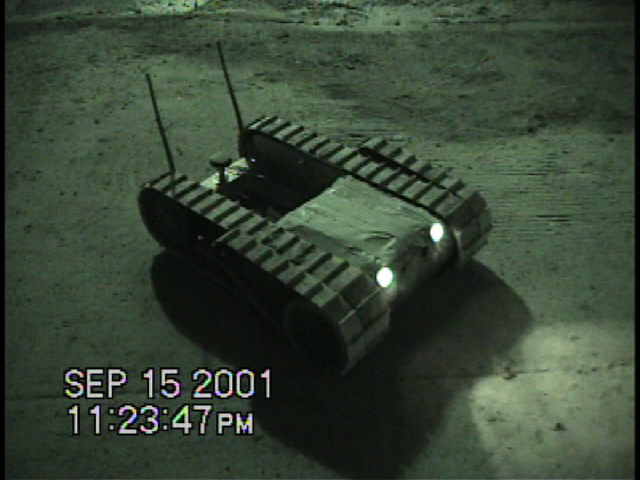
\includegraphics[width=8cm]{./figs/packbot.jpg}
        \par\medskip
Fonte: https://nsf.gov/news/mmg/media/images/packbot6\_f\_7e432d6d-ab16-4b4f-8944-0d89a8bef999.jpg
        \label{fig:packbot}
\end{figure}

O terremoto e tsunami que atingiram o Japão em 2011 teve grande impacto na Central Nuclear de \textit{Fukushima Daiichi}. A perda de energia devido ao desastre natural gerou explosões de hidrogênio na usina nuclear, na qual três reatores foram danificados. Em um deles, os danos foram tão profundos, que houve vazamento de material radioativo, com possível contaminação do Oceano Pacífico. Devido ao alto nível de radiação, não seria possível intervenção humana sem que houvesse riscos de vida.
Desse modo, para poder analisar os danos existentes dentro da usina nuclear e conter o vazamento de água contaminada o uso de um dispositivo remotamente controlado era indispensável.
Em um cenário de urgência, a \textit{New Energy and Industrial Technology Development Organization} (NEDO) e a \textit{}{Tokyo Electric Power Company (TEPCO)} juntaram esforço no projeto do robô Quince, mostrado na figura \ref{fig:quince}, que atuou nas missões na Usina Nuclear de \textit{Fukushima Daiichi} \cite{nagatani2013emergency}.

 \begin{figure}[H]  
        \centering
        \caption{Robô \textit{}{Quince} que atuau nas 6 missões de Usina Nuclear de \textit{Fukushima Daiichi}.}
        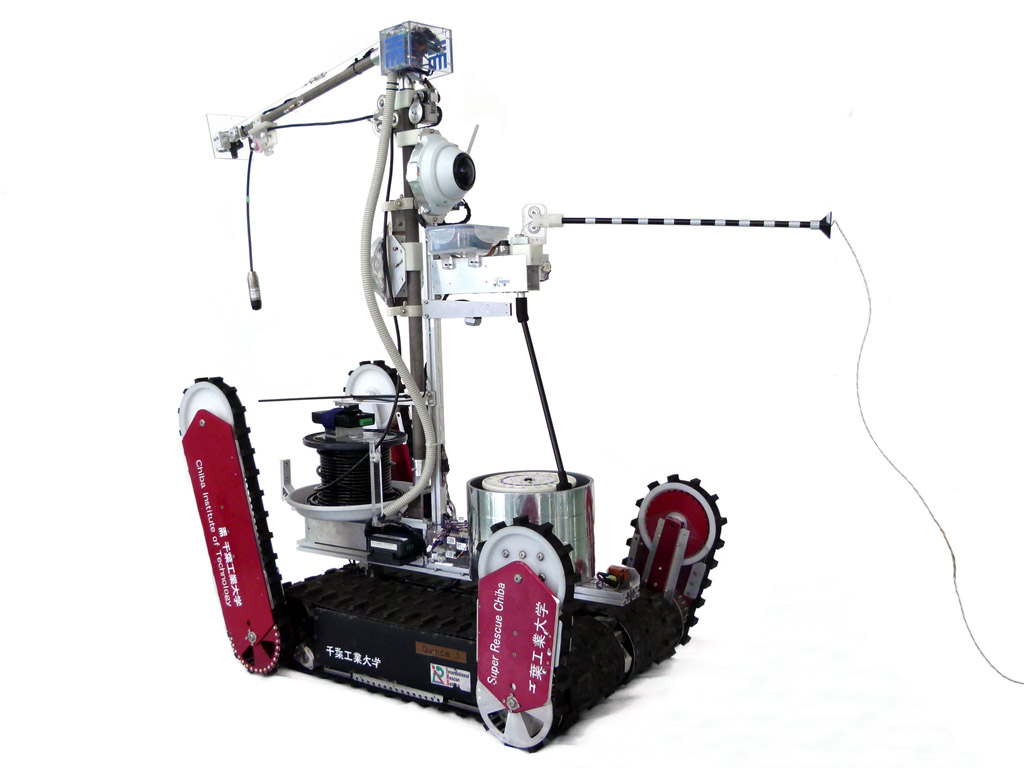
\includegraphics[width=8cm]{./figs/quince.jpg}
        \label{fig:quince}
\end{figure}

Em 2019, durante o incêndio na catedral de \textit{Notre Dame}, um robô remotamente controlado chamado de \textit{Colossus}, mostrado na figura \ref{fig:colossus2019}, foi utilizado para extinguir chamas de áreas que poderiam comprometer a vida de bombeiros\cite{colossus2019}.

 \begin{figure}[h]  
        \centering
        \caption{Robô \textit{}{Colossus} utilizado no controle de chamas.}
        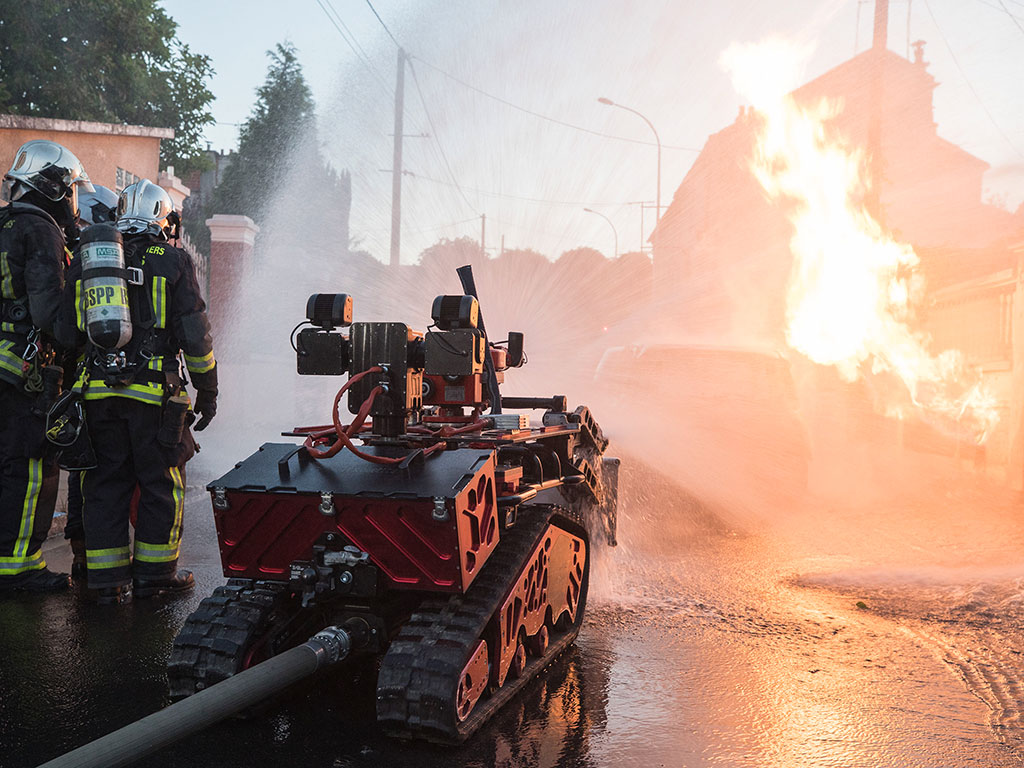
\includegraphics[width=8cm]{./figs/colossus2019.jpg}
        \par\medskip
Fonte: https://robots.ieee.org/robots/quince/
        \label{fig:colossus2019}
\end{figure}
%https://robots.ieee.org/robots/colossus/

%https://builtin.com/robotics/rescue-robots

No mesmo ano, a \textit{Boston Dynamics} apresentou a nova versão de seu robô humanoide, \textit{Atlas}, mostrado na figura \ref{fig:atlas}. Diferentemente dos outros robôs, destacados previamente, o \textit{Atlas} possui alta mobilidade, podendo se locomover eficientemente em diferentes terrenos além de segurar objetos \cite{atlas}.

 \begin{figure}[H]  
        \centering
        \caption{Robô \textit{Atlas} da \textit{Boston Dynamics}.}
        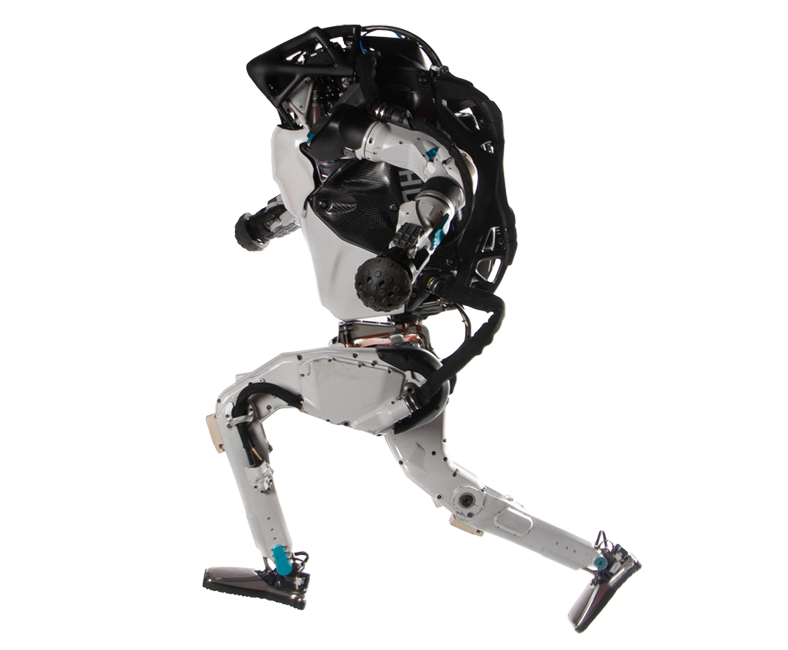
\includegraphics[width=8cm]{./figs/atlas.png}
        \par\medskip
Fonte: https://www.bostondynamics.com/atlas
        \label{fig:atlas}
\end{figure}

Uma das dificuldades do uso de robôs em missões de resgate esta no transporte desses dispositivos para suas área de atuação. No caso de terremotos, a obstrução de vias pode dificultar o acesso terrestre, que já é um obstáculo para as equipes médicas. Umas possível solução esta no transporte aéreo, na qual robôs podem ser enviados em aviões ou helicópteros e entregados por meio de paraquedas.
Esta solução possui alguns obstáculos a serem superados, um deles se encontra durante a fase de aterrissagem. Mesmo com a desaceleração proveniente do paraquedas, o impacto ao solo ainda é alto. Com uma força de aterrissagem média de 11$kN$, o risco de lesão é de 6 a cada 1000 aterrissagens, podendo aumentar quando a aterrissagem é feita incorretamente \cite{whitting2007parachute}.
Para robôs, essas lesões se traduzem como danos ao equipamentos e componentes frágeis, como visto em \cite{tsujita2017drop}.
Estudos realizados com robôs de uma perna, mostraram uma redução na aceleração de impacto quando uma postura semi-sentada é adotada\cite{tsujita2017drop}. Adicionalmente,
breves estudos mostraram a performance do uso de materiais acolchoados na redução das acelerações de impacto ao solo \cite{tsujita2017drop} \cite{tsujita2017analysis}.
Desse modo, mostra-se interessante a continuidade deste trabalho, com uma análise mais profundada no uso de materiais acolchoados em testes de queda. Adicionalmente, a construção de um simulador de testes de queda se mostra essencial, uma vez que os experimentos nas pesquisas mencionadas são realizados a um alto custo financeiro. Realizar repetidos testes de queda em robôs humanoides é inviável dado a perspectiva de danificá-los devido ao impacto ao solo, como mostrado em \cite{tsujita2017drop}.

%https://singularityhub.com/2019/04/12/ai-and-robotics-are-transforming-disaster-relief/

%https://builtin.com/robotics/rescue-robots

%https://onlinelibrary.wiley.com/doi/full/10.1046/j.1442-2026.2001.00201.x

%https://journals.lww.com/co-criticalcare/fulltext/2005/12000/Disaster_management_teams.13.aspx

%https://www.student.cs.uwaterloo.ca/~cs492/papers/trial.pdf

\section{Objetivos}

Este trabalho tem como objetivo a análise do envio de robôs humanoides em áreas de baixa acessibilidade terrestre utilizando aterrissagem por paraquedas e materiais acolchoados para reduzir as acelerações de impacto.
Como objetivos específicos, têm-se modelar um simulador dinâmico para o experimentos de testes de queda, analisar o desempenho dos amortecimentos em reduzir as acelerações de impacto e identificar os parâmetros de Rayleigh para os materiais utilizados nos testes de queda.

\section{Materiais e Métodos}

O trabalho se inicia com uma contextualização, justificando o problema a ser estudado, apresentando estudos e pesquisas relevantes sobre o tema.
A seguir, serão apresentados aspectos gerais \textit{Métodos dos Elementos Finitos} (MEF) e \textit{Dinâmica de Multicorpos} que vão possibilitar o leitor compreender o simulador dinâmico de teste de queda, que será desenvolvido neste trabalho.
Experimentos serão desenvolviods com o objetivo de calibrar e validar o simulador criado.
Gráficos e tabelas serão utilizados para mostrar os resultados.

\section{Organização do Trabalho}

Este trabalho está divido em 6 capítulos, com a seguinte divisão:

O capítulo 1 se inicia com uma breve introdução da justificativa, do problema a ser estudado e trabalhos importantes sobre o tema. No decorrer deste capítulo, os temas são devidamente aprofundados.

No capítulo 2 e capítulo 3, a dinâmica de multicorpos e o MEF são, respectivamente, introduzidos, de modo a fornecer ao leitor as ferramentas fundamentais para compreensão da ferramenta apresentada no capítulo seguinte. 

No capítulo 4 será descrito o simulador dinâmico de teste de queda implementado no \textit{Matlab/Simulink}.

No capítulo 5 será descrito o experimento de teste de queda, utilizando para calibrar a ferramenta mencionada no capítulo 4.

No capítulo 6, serão apresentados os resultados e as conclusões deste trabalho.








\chapter{Dinâmica de Multi-Corpos}\label{cap:multicorpos}


\chapter{Métodos dos Elementos Finitos}\label{cap:elementosfinitos}

O MEF é uma ferramenta de simulação empregada em diversos campos da engenharia, sendo utilizada desde a análise de sólidos e estruturas à transferência de calor e fluidos \cite{bathe2006finite}. 

Como existe uma gama de materiais publicados sobre esse tema, este capítulo irá apresentá-lo resumidamente, de modo a possibilitar a compreensão do trabalho realizado no capítulo 5. Para um aprofundamento sobre o MEF, \cite{bathe2006finite}, \cite{felippa2004introduction} e \cite{felippa2003advanced} são leituras recomendadas.

Na análise pelo MEF,uma aproximação da variável de interesse é definida, por meio de funções de interpolação dos valores incógnitos dessas variáveis, posteriormente, a estrutura é discretizada como sendo composta por elementos finitos, formados por arestas conectadas a vértices por meio de nós. Um sistema de equações discretas é obtido e após aplicar condições de contorno, os valores das variáveis de interesse são obtidos e o comportamento geral da estrutura foi então simulado/aproximado.

Desse modo, para simular o comportamento do material acolchoado durante o impacto no teste de queda, mostrado na figura \ref{fig:CorpoDeProva}, é realizado uma subdivisão desse material em elementos tetraédricos, sendo cada um formado por 4 nós. A malha resultante é mostrada na figura \ref{fig:ElementoFinito}. 

 \begin{figure}[H]  
        \centering
        \caption{Corpo de prova com material acolchoado.}
        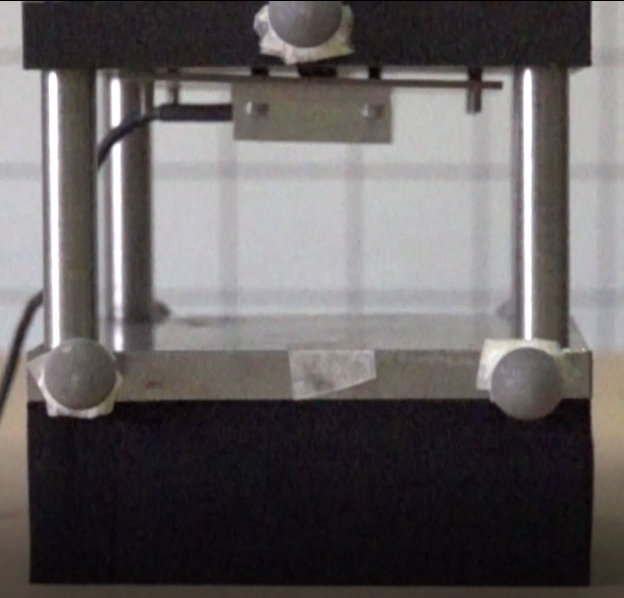
\includegraphics[width=8cm]{./figs/CorpoDeProva.PNG}
        \par\medskip
        Fonte: Própria autoria.
        \label{fig:CorpoDeProva}
\end{figure}

 \begin{figure}[H]  
        \centering
        \caption{Material acolchoado sendo modelado por uma malha tetraédrica.}
        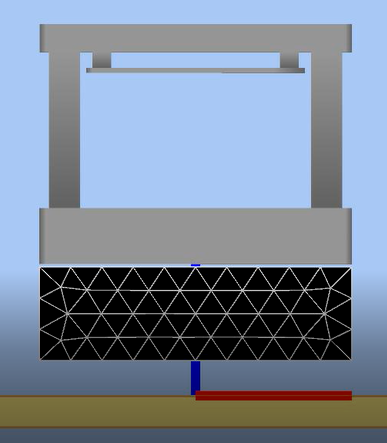
\includegraphics[width=8cm]{./figs/MaterialDividido.PNG}
        \par\medskip
        Fonte: Própria autoria.
        \label{fig:ElementoFinito}
\end{figure}


Conforme \cite{Chen2017numerical}, para o elemento tetraédrico, mostrado na figura \ref{fig:finiteelement}, as coordenadas e deslocamentos, medidos nas coordenadas locais, dos nós 1, 2, 3 e 4 são, respectivamente, $(x_{i}, y_{i}, z_{i})$ e $(u_{i}, v_{i}, w_{i})$, para $i = {1, 2, 3, 4}$.

 A função de otimização que determina o deslocamento $(u, v, w)$ do ponto $(x, y, z)$ é expressa da seguinte maneira:
 
 %funcao de interpolacao linear
 
 \begin{figure}[h]  
        \centering
        \caption{Deslocamento dos nós para um elemento tetraédrico. \cite{Chen2017numerical}.}
        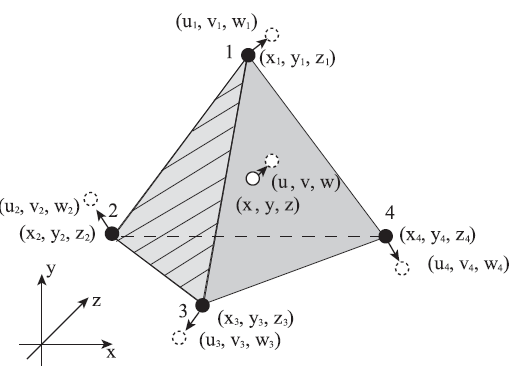
\includegraphics[width=8cm]{./figs/finiteelement.png}
        \label{fig:finiteelement}
\end{figure}

\begin{equation}
\label{eqn:interpolation}
\begin{aligned}
u &= \alpha_{1} + \alpha_{2}x + \alpha_{3}y + \alpha_{4}z, \\
v &= \alpha_{5} + \alpha_{6}x + \alpha_{7}y + \alpha_{8}z, \\
w &= \alpha_{9} + \alpha_{10}x + \alpha_{11}y + \alpha_{12}z
\end{aligned}
\end{equation}

Neste trabalho, o material estudado é considerado isotrópico, homogêneo e com deformação linear. Sob essas hipóteses, as deformações de engenharia $\epsilon_{e} = (\epsilon_{x}, \epsilon_{y}, \epsilon_{z}, \gamma_{xy}, \gamma_{yz}, \gamma_{zx})$, são definidas da seguinte forma:

\begin{equation} \label{eq:axialdef}
    \begin{aligned}
    &\epsilon_{x} = \frac{\partial u}{\partial x}, 
    &\epsilon_{y} = \frac{\partial v}{\partial y}, 
    &\epsilon_{z} = \frac{\partial w}{\partial z}
    \end{aligned}
\end{equation}

\begin{equation} \label{eq:angulardef}
    \begin{aligned}
    &\gamma_{xy} = \frac{\partial u}{\partial y} + \frac{\partial v}{\partial x}, 
    &\gamma_{yz} = \frac{\partial v}{\partial z} + \frac{\partial w}{\partial y}, 
    &\gamma_{zx} = \frac{\partial w}{\partial x} + \frac{\partial u}{\partial z}
    \end{aligned}
\end{equation}

Por meio da Lei de Hooke, as deformações podem ser reescritas da seguinte forma:

\begin{equation} \label{eq:tensaodeformacao1}
    \begin{aligned}
        \epsilon_{x} = \frac{\sigma_{x} - \nu(\sigma_{y} + \sigma_{z})}{E},
        \epsilon_{y} = \frac{\sigma_{y} - \nu(\sigma_{z} + \sigma_{x})}{E},
        \epsilon_{z} = \frac{\sigma_{z} - \nu(\sigma_{x} + \sigma_{y})}{E}
    \end{aligned}    
\end{equation}
\begin{equation} \label{eq:tensaodeformacao2}
    \begin{aligned}
        \gamma_{xy} = \frac{\uptau_{xy}}{G},
        \gamma_{yz} = \frac{\uptau_{yz}}{G},
        \gamma_{zx} = \frac{\uptau_{zx}}{G}
    \end{aligned}
\end{equation}
onde $E$, $G$ e $\nu$ são, respectivamente, Módulo de Young, Módulo de Cisalhamento e Coeficiente de Poisson.

Das equações \ref{eqn:interpolation}, \ref{eq:axialdef} e \ref{eq:angulardef}, \ref{eq:tensaodeformacao1} e \ref{eq:tensaodeformacao2} obtêm-se as seguintes relações matriciais:

\begin{equation} \label{eq:matrixdisplacement}
    \begin{Bmatrix}
        u_{1} \\
        v_{1} \\
        w_{1} \\
        u_{2} \\
        v_{2} \\
        w_{2} \\
        u_{3} \\
        v_{3} \\
        w_{3} \\
        u_{4} \\
        v_{4} \\
        w_{4} \\
    \end{Bmatrix}
    = 
    \begin{bmatrix}
    1 & x_{1} & y_{1} & z_{1} & 0 & 0 & 0 & 0 & 0 & 0 & 0 & 0 \\
    0 & 0 & 0 & 0 &  1 & x_{1} & y_{1} & z_{1} & 0 & 0 & 0 & 0 \\
    0 & 0 & 0 & 0 & 0 & 0 & 0 & 0 & 1 & x_{1} & y_{1} & z_{1} \\
    1 & x_{2} & y_{2} & z_{2} & 0 & 0 & 0 & 0 & 0 & 0 & 0 & 0 \\
    0 & 0 & 0 & 0 &  1 & x_{2} & y_{2} & z_{2} & 0 & 0 & 0 & 0 \\
    0 & 0 & 0 & 0 & 0 & 0 & 0 & 0 & 1 & x_{2} & y_{2} & z_{2} \\
    1 & x_{3} & y_{3} & z_{3} & 0 & 0 & 0 & 0 & 0 & 0 & 0 & 0 \\
    0 & 0 & 0 & 0 &  1 & x_{3} & y_{3} & z_{3} & 0 & 0 & 0 & 0 \\
    0 & 0 & 0 & 0 & 0 & 0 & 0 & 0 & 1 & x_{3} & y_{3} & z_{3} \\
    1 & x_{4} & y_{4} & z_{4} & 0 & 0 & 0 & 0 & 0 & 0 & 0 & 0 \\
    0 & 0 & 0 & 0 &  1 & x_{4} & y_{4} & z_{4} & 0 & 0 & 0 & 0 \\
    0 & 0 & 0 & 0 & 0 & 0 & 0 & 0 & 1 & x_{4} & y_{4} & z_{4} \\
    \end{bmatrix}
    \begin{Bmatrix}
        \alpha_{1} \\
        \alpha_{2} \\
        \alpha_{3} \\
        \alpha_{4} \\
        \alpha_{5} \\
        \alpha_{6} \\
        \alpha_{7} \\
        \alpha_{8} \\
        \alpha_{9} \\
        \alpha_{10} \\
        \alpha_{11} \\
        \alpha_{12} \\
    \end{Bmatrix}
\end{equation}

\begin{equation} \label{eq:matrixalphadisplacement}
    \begin{Bmatrix}
        \epsilon_{x} \\
        \epsilon_{y} \\
        \epsilon_{z} \\
        \gamma_{xy} \\
        \gamma_{yz} \\
        \gamma_{zx} \\
    \end{Bmatrix}
    = 
    \begin{bmatrix}
    0 & 1 & 0 & 0 & 0 & 0 & 0 & 0 & 0 & 0 & 0 & 0 \\
    0 & 0 & 0 & 0 & 0 & 0 & 1 & 0 & 0 & 0 & 0 & 0 \\
    0 & 0 & 0 & 0 & 0 & 0 & 0 & 0 & 0 & 0 & 0 & 1 \\
    0 & 0 & 1 & 0 & 0 & 1 & 0 & 0 & 0 & 0 & 0 & 0 \\
    0 & 0 & 0 & 0 & 0 & 0 & 0 & 1 & 0 & 0 & 1 & 0 \\
    0 & 0 & 0 & 1 & 0 & 0 & 0 & 0 & 0 & 1 & 0 & 0 \\
    \end{bmatrix}
    \begin{Bmatrix}
        \alpha_{1} \\
        \alpha_{2} \\
        \alpha_{3} \\
        \vdots \\
        \alpha_{11} \\
        \alpha_{12} \\
    \end{Bmatrix}
\end{equation}

\begin{equation} \label{eq:elasticitymatrix}
    \begin{Bmatrix}
        \sigma_{x} \\
        \sigma_{y} \\
        \sigma_{z} \\
        \uptau_{xy} \\
        \uptau_{yz} \\
        \uptau_{zx} \\
    \end{Bmatrix} 
    =
    \frac{E(1 - \nu)}{(1+\nu)(1 - 2\nu)}
    \begin{bmatrix}
        1 & \frac{\nu}{1-\nu} & \frac{\nu}{1-\nu} & 0 & 0 & 0 \\
        \frac{\nu}{1-\nu} & 1 & \frac{\nu}{1-\nu} & 0 & 0 & 0 \\
        \frac{\nu}{1-\nu} & \frac{\nu}{1-\nu} & 1 & 0 & 0 & 0 \\
        0 & 0 & 0 & \frac{1-2\nu}{2(1-\nu)} & 0 & 0 \\
        0 & 0 & 0 & 0 & \frac{1-2\nu}{2(1-\nu)} & 0 \\
        0 & 0 & 0 & 0 & 0 & \frac{1-2\nu}{2(1-\nu)} \\
    \end{bmatrix}
    
    \begin{Bmatrix}
        \epsilon_{x}\\
        \epsilon_{y}\\
        \epsilon_{z}\\
        \gamma_{xy}\\
        \gamma_{yz}\\
        \gamma_{zx}\\
    \end{Bmatrix}
\end{equation}

Na forma compacta, tem-se, respectivamente,

\begin{equation} \label{eq:simplifiedeq}
    \begin{aligned}
      \pmb{u_{e}} &= \pmb{A}\alpha, \\
      \epsilon_{e} &= \pmb{B}\alpha, \\
      \pmb{\delta_{e}} &= \pmb{C}_{e} \epsilon_{e}
    \end{aligned}
\end{equation}
onde $\pmb{A}$ é a matriz dos coeficientes de deslocamento dos nós e
$\pmb{C}_{e}$ é a matriz de elasticidade. A matriz $B_{e}$, chamada de matriz de tensão-deformação, é definida como $\pmb{B}_e = \pmb{B}\pmb{A}^{-1}$.

Do princípio do trabalho virtual, a matriz de rigidez de um elemento,  $\pmb{K}_{e}$, é definido como:

\begin{equation} \label{eq:elementrig}
    \pmb{K}_{e} = \pmb{B}^{T}_{e}\pmb{C}_{e}\pmb{B}_{e}V_{e} 
\end{equation}
onde $\pmb{C}_{e}$ e $\pmb{B}_{e}$ são as matrizes definidas previamente, e $V_{e}$ é o volume do elemento finito. Para um elemento tetraédrico, o volume depende das coordenadas dos 4 nós e é dado por:

\begin{equation} \label{eq:volume}
V_{e} = \frac{1}{6} 
\begin{vmatrix}
 1 & 1 & 1 & 1 \\
 x1 & x2 & x3 & x4 \\
 y1 & y2 & y3 & y4 \\
 z1 & z2 & z3 & z4 
\end{vmatrix}
\end{equation}

A partir da matriz de rigidez de cada elemento $\pmb{K}_{e}$, a matriz de rigidez global da estrutura, $\pmb{K}$ é calculada.

Para maior detalhamento das deduções realizadas neste capítulo, consultar \cite{Chen2017numerical}.

Na análise dinâmica de estruturas, equação que governa o deslocamento dos $N$ nós de uma malha, conforme \cite{hughes2012finite}, é dada por:

\begin{equation} \label{eq:dynamic}
\pmb{M}\ddot{\pmb{u}} + \pmb{D}\dot{\pmb{u}} + \pmb{K}\pmb{u} = \pmb{f} 
\end{equation}
onde $u$ é o vetor de deslocamento de ordem $N$, $\dot{u}$ e $\ddot{u}$ são, respectivamente, a primeira e segunda derivadas temporais de $u$.

$\pmb{K}$ representa a matriz de rigidez global da estrutura, descrita previamente.

$\pmb{M}$ representa a matriz de massa da estrutura. 
Diversos métodos podem ser utilizados no cálculo da matriz de massa, entretanto dois métodos se destacam, sendo amplamente citados na literatura: a matriz de massa consistente ("Consistent Mass Matrix")  e a matriz de massa concentrada ("Lumped Mass Matrix") \cite{felippa2004introduction}.

%Explicar Consistent Mass Matrix

%Explicar Lumped Mass Matrix

O MEF é um método numérico, assim as soluções obtidas apresentam um erro e sua magnitude depende de alguns fatores. Por exemplo, como a análise de um objeto contínuo é feita por meio de um modelo discreto, a magnitude do erro é influenciada pelo formato do elemento finito ou do nível de refinamento da malha. Ao se utilizar elementos finitos cada vez menores, o MEF tende a soluções mais próximas da solução exata, quando existem, entretanto, aumenta-se o custo computacional envolvido. 
A utilização da matriz de massa concentrada é interessante pois a matriz de massa resultante é diagonal, o que simplifica o custo-computacional envolvido no cálculo de sua inversa, $\pmb{M}^{-1}$.
Por outro lado, a matriz de massa consistente apresenta resultados mais precisos. Entretanto, o tamanho dos elementos escolhido deve ser pequeno, elevando o custo computacional envolvido \cite{Chen2017numerical}.

Para este trabalho, a matriz de massa concentrada é utilizada, uma vez que a malha escolhida não possui elementos finitos pequenos o suficiente que torne o resultado com a matriz de massa consistente mais preciso do que a matriz de massa concentrada. Além disso, a matriz de massa concentrada destaca-se pela relativa simplicidade de aplicação e menor custo-computacional envolvido.

A matriz de massa concentrada $\pmb{M}$, conforme \cite{Chen2017numerical}, é definida como:

\begin{equation} \label{eq:massmatrix}
    \pmb{M} = 
    \begin{pmatrix}
    \pmb{m}_{1} &        &   &    &  \\
                & \ddots &   &  0 &  \\
                &        & \pmb{m}_{i} & & \\
                & 0      &             &  \ddots &\\
                & & & & \pmb{m}_{n}
    \end{pmatrix}
\end{equation}

\begin{equation} \label{eq:mass}
\pmb{m}_{i} =
\begin{pmatrix}
    m_{i} & 0 & 0 \\
    0 & m_{i} & 0 \\
    0 & 0 & m_{i} \\
\end{pmatrix}
\end{equation}
\begin{equation}
    m_{i} = \sum_{j=1}^{N_{ij}} \frac{\rho V_{j}}{4}    
\end{equation}
onde $m_{i}$ é a massa concentrada nó, $\rho$ é a densidade e $V_{j}$ o volume do elemento $j$. $N_{ij}$ é o número de elementos que compartilhar o nó $j$.

$\pmb{D}$ representa a matriz de amortecimento. O amortecimento é utilizado para caracterizar a energia dissipada pelo material acolchoado durante o impacto de queda \cite{ge2018impact}. Será utilizado um modelo viscoso linear, no qual a força de amortecimento é proporcional linearmente à velocidade de deformação. 

Para sistemas de múltiplos graus de liberdade, a teoria de amortecimento ainda não é bem estabelecida. Uma das razões reside na dificuldade em se obter informações sobre o amortecimento de um sistema para o calculo da matriz $\pmb{D}$ \cite{liu1995formulation}.
Uma aproximação comumente aplicada é o amortecimento de Rayleigh, definido como:

\begin{equation} \label{eq:damping}
\pmb{D} = \alpha \pmb{M} + \beta \pmb{K}
\end{equation}
onde $\pmb{M}$ e $\pmb{K}$ são, respectivamente, as matrizes de massa e rigidez, $\alpha$ e $\beta$ são os parâmetros de Rayleigh, constantes arbitrárias obtidas experimentalmente, pois variam de acordo com o design da estrutura e o material aplicado. Além disso, esses parâmetros não possuem significado físico, sendo utilizados apenas para estabilização de cálculo \cite{Chen2017numerical}.

A Eq. \ref{eq:dynamic} apresentada anteriormente é dependente do tempo, de modo que, para uma análise dinâmica do sistema, é necessário a sua resolução para todo instante de tempo $t$. Para a solução, será utilizado o método de integração numérica de Newmark, conforme apresentado em \cite{bathe2006finite}.

Assim como foi fundamental, para a análise da estrutura, discretiza-la em elementos menores através do MEF, para a análise dinâmica do sistema, a discretização do tempo também deve ser feita.
Para um intervalo de tempo de $0$ a $T$, $T$ é divido em $n$ intervalos iguais de tempo $\Delta t$, ou seja $\Delta t = T/n$, assim, a integração da Eq.\ref{eq:dynamic} resulta em soluções aproximadas para cada instante de tempo $\Delta t, 2\Delta t, 3\Delta t, ..., T$.
Como o método empregado calcula a solução no próximo instante de tempo, são utilizadas as soluções obtidas nos instantes $0, \Delta t, 2\Delta t, ..., t$, para calcular a solução em $t + \Delta t$. Além disso, condições iniciais $u_{0}$, $\dot{u}_{0}$ e $\ddot{u}_{o}$ em $t = 0$, são assumidas como conhecidas.

Escrevendo a Eq.\ref{eq:dynamic} no instante $t + \Delta t$ tem-se:

\begin{equation} \label{eq:dynamic_timestep}
\pmb{M}\ddot{\pmb{u}}_{t + \Delta t} + \pmb{D}\dot{\pmb{u}}_{t + \Delta t} + \pmb{K}\pmb{u}_{t + \Delta t} = \pmb{f}_{t + \Delta t}
\end{equation}

No método de integração Newmark, o deslocamento e a velocidade no instante $t + \Delta t$ é dado por:

\begin{equation}\label{eq:newmark_velocity}
\dot{\pmb{u}}_{t + \Delta t} = \dot{\pmb{u}}_{t} + \left[\left(1 - \delta\right)\ddot{\pmb{u}}_{t} + \delta \ddot{\pmb{u}}_{t + \Delta t} \right]
\end{equation}

 \begin{equation}\label{eq:newmark_displacement}
\pmb{u}_{t + \Delta t} = \pmb{u}_{t} + \dot{\pmb{u}}_{t}\Delta t + \left[\left(\frac{1}{2} - \alpha\right) \ddot{\pmb{u}}_{t} + \alpha \ddot{\pmb{u}}_{t + \Delta  t}\right] \Delta t^{2}
\end{equation}

Isolando o termo $\ddot{\pmb{u}}_{t+\Delta t}$ da Eq. \ref{eq:newmark_displacement}, tem-se:

\begin{equation}\label{eq:newmark_disp_acc}
\ddot{\pmb{u}}_{t + \Delta t} = \frac{1}{\alpha}\left[\left(\alpha - 1/2\right)\ddot{\pmb{u}}_t + \frac{\pmb{u}_{t + \Delta t} - \pmb{u}_{t} - \dot{\pmb{u}}_{t}\Delta t }{\Delta t^{2}}\right]
\end{equation}

Substituindo \ref{eq:newmark_disp_acc} na Eq.\ref{eq:newmark_velocity}:

\begin{equation}\label{eq:newmark_vel_acc}
\dot{\pmb{u}}_{t + \Delta t} = \dot{\pmb{u}}_{t} + \frac{1}{\Delta t}\left[\left(1-\delta\right)\ddot{\pmb{u}}_{t} + \frac{\delta}{\alpha}\left[\left(\alpha - 1/2\right)\ddot{\pmb{u}}_{t} + \frac{\pmb{u}_{t + \Delta t} - \pmb{u}_{t} - \dot{\pmb{u}}_{t}\Delta t }{\Delta t^{2}} \right]\right]
\end{equation}

Substituindo \ref{eq:newmark_disp_acc} e \ref{eq:newmark_vel_acc} na Eq.\ref{eq:dynamic_timestep} e isolando o termo $\pmb{u}_{t + \Delta t}$:

\begin{equation}\label{eq:newmark_geral}
\begin{split}
\left(\frac{1}{\alpha \Delta t^{2}}\pmb{M} + \frac{\delta}{\alpha \Delta t} \pmb{D} + \pmb{K}\right) \pmb{u}_{t + \Delta t} = \pmb{f}_{t + \Delta t} + \left[\left(\frac{1}{2\alpha} - 1\right) \ddot{\pmb{u}}_{t} + \frac{1}{2\Delta t}\dot{\pmb{u}}_{t} + \frac{1}{\alpha \Delta t^{2}}\right]\pmb{M} \\
+ \left[\left(\alpha + \frac{\delta}{2\alpha} - \delta - 1\right)\ddot{\pmb{u}}_{t} + \left(2 - \frac{\delta}{\alpha}\right)\dot{\pmb{u}}_{t} + \frac{\delta}{\alpha\Delta t}\pmb{u}_{t}\right]\pmb{D}
\end{split}
\end{equation}

Onde $\alpha$ e $\delta$ são parâmetros utilizados para estabilizar a integração e ajustar sua precisão. Newmark propôs originalmente os valores $\alpha = \frac{1}{4}$ e $\delta = \frac{1}{2}$ para que o método seja incondicionalmente estável \cite{bathe2006finite}.

Utilizando os dados propostos por Newmark, a Eq. \ref{eq:newmark_geral} torna-se:

\begin{equation}\label{eq:newmark_specific}
\left(\frac{4}{\Delta t^{2}}\pmb{M} + \frac{2}{\Delta t} \pmb{D} + \pmb{K}\right) \pmb{u}_{t + \Delta t} = \pmb{f}_{t + \Delta t} + \left(\ddot{\pmb{u}}_{t} + \frac{4}{\Delta t}\dot{\pmb{u}}_{t} + \frac{4}{\Delta t^{2}}\pmb{u}_{t}\right)\pmb{M} + \left(\dot{\pmb{u}}_{t} + \frac{2}{\Delta t}\pmb{u}_{t}\right)\pmb{D}
\end{equation}

 A partir da Eq. \ref{eq:newmark_specific} $\pmb{u}_{t + \Delta t}$ é calculado. Em seguida, $\ddot{\pmb{u}}_{t + \Delta t}$ e $\dot{\pmb{u}}_{t + \Delta t}$ são obtidos pelas equações \ref{eq:newmark_disp_acc} e \ref{eq:newmark_vel_acc}.
 


\chapter{Testes de Queda}\label{cap:testesdequeda}

\section{Ensaios Experimentais}

Neste capítulo será apresentado a metodologia dos experimentos de teste de queda. Os experimentos foram realizados no Instituto de Tecnologia de Shibaura e na Academia de Defesa Nacional, ambos localizados no Japão, sob supervisionamento dos professores Satoko Abiko e Teppei Tsujita.

O corpo de prova consiste em uma armação retangular com $35mm$ de altura e $100mm$ de largura e comprimento. A armação tem como função proteger e permitir a fixação dos acelerômetros utilizados durante o experimento.
Para garantir uma correta aquisição dos dados e evitar a saturação das acelerações de impacto, dois tipos diferentes de sensores foram utilizados.
No teste com material acolchoado macio, foram aplicados um micro-computador \textit{Intel Edison} e um kit de módulos da \textit{Sparkfun}. O Intel Edison, mostrado na figura \ref{fig:edison}, é equipado com um processador dual-core \textit{Intel Atom} e realiza a comunicação com o módulo 9DoF, equipado com um acelerômetro IMU LSM9DS0, o qual possui uma resolução de $16g$ e uma frequência de $1kHz$.

 \begin{figure}[H]  
        \centering
        \caption{ \textit{Intel Edison} acoplado aos módulos da \textit{Sparkfun}}
        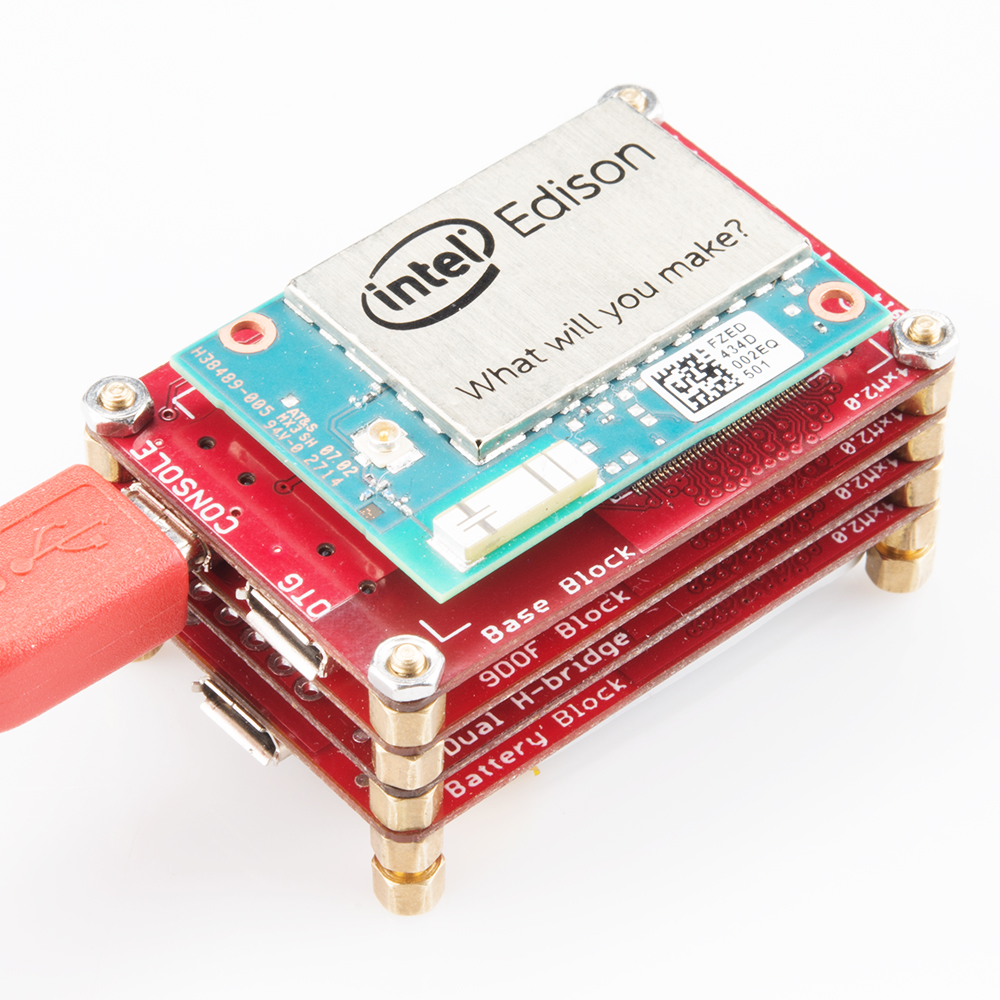
\includegraphics[width=8cm]{./figs/intel_edison.jpg}
        \par\medskip
        Fonte: https://learn.sparkfun.com/tutorials/general-guide-to-sparkfun-blocks-for-intel-edison/all
        \label{fig:edison}
        %https://learn.sparkfun.com/tutorials/general-guide-to-sparkfun-blocks-for-intel-edison/all
\end{figure}

Para o teste com material acolchoado rígido, foi utilizado o acelerômetro da \textit{Microstone} modelo MA3-50AD, mostrado na figura \ref{fig:microstone},  que possui uma resolução de $50g$ a uma frequência de $1kHz$.

 \begin{figure}[H]  
        \centering
        \caption{ Acelerômetro MA3-50AD da \textit{Microstone}.}
        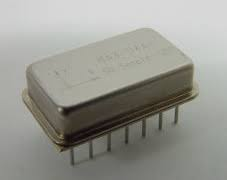
\includegraphics[width=8cm]{./figs/microstone.jpeg}
        \par\medskip
        Fonte: http://microstonecorp.sakura.ne.jp/wp/wp-content/uploads/2018/04/MA3\_R31.pdf
        \label{fig:microstone}
\end{figure}

Na face superior, uma chapa de metal foi fixada de modo a possibilitar a suspensão do corpo de teste por um eletroímã. já na face inferior, foram fixados os materiais acolchoados que seriam submetidos para análise. Adicionalmente, 6 pequenas esferas cinza foram coladas ao redor do corpo de teste. Por meio de 6 câmeras de captura de movimento, o software \textit{Optitrack:Motive} monitora a posição das esferas cinzas. Desse modo, tanto a aceleração como a posição do dispositivo são obtidos durante o ensaio experimental.

O dispositivos descritos são mostrados nas figuras \ref{fig:CorpoDeProva2} e \ref{fig:SoftCorpo} a seguir:

 \begin{figure}[H]  
        \centering
        \caption{Corpo de prova com material acolchoado rígido contendo os marcadores esféricos cinzas e, no centro da estrutura, o acelerômetro MA3-50AD da \textit{Microstone}.}
        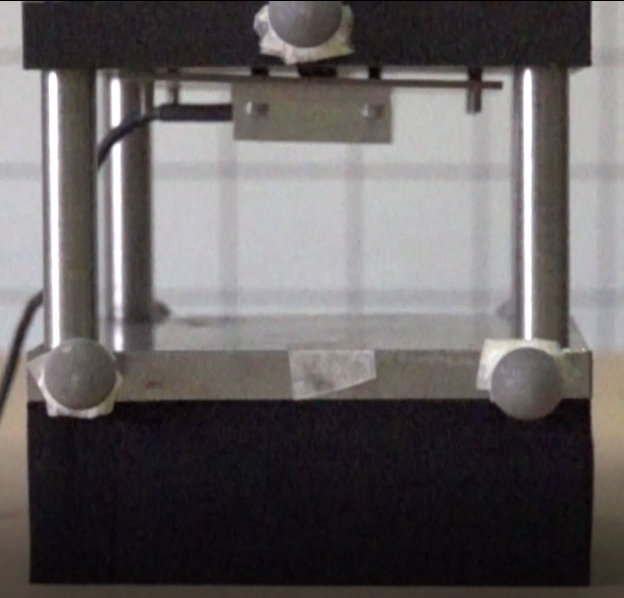
\includegraphics[width=8cm]{./figs/CorpoDeProva.PNG}
        \par\medskip
        Fonte: Própria autoria.
        \label{fig:CorpoDeProva2}
\end{figure}

 \begin{figure}[H]  
        \centering
        \caption{Corpo de prova com material acolchoado macio, pode-se observar os marcadores esféricos cinzas fixados na estrutura, a chapa metálica no topo do dispositivo e no centro, o conjunto \textit{Intel Edison} e os módulos para aquisição de dados.}
        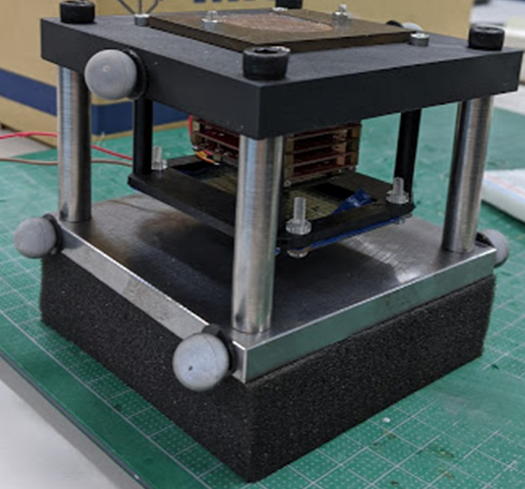
\includegraphics[width=8cm]{./figs/soft_drop_test.PNG}
        \par\medskip
        Fonte: Própria autoria.
        \label{fig:SoftCorpo}
\end{figure}

Duas câmeras foram utilizadas para a captura visual do experimento. A primeira, a câmera \textit{Sony HDR-CX900} foi utilizada para a filmagem e gravação do áudio de uma visão ampla do experimento. A segunda, \textit{Sony RX100M5}, é uma câmera \textit{High Frame Rate} (HFR) utilizada para produzir vídeos em câmera lenta, sendo capaz de registaté 960 quadros por segundo \cite{sonyHFR}. Ela foi utilizada para capturar a deformação do material acolchoado durante o impacto ao solo.

Para cada material acolchoado, foram realizados testes de queda utilizando alturas de $5cm$ e $8cm$. O dispositivo suspendido foi por um eletroímã, alimentado por uma fonte de tensão DC. Um goniômetro digital foi utilizado para garantir que o solo e a face inferior do corpo de prova estivessem paralelas. Para reduzir o impacto e proteger os dispositivos eletrônicos utilizados durante o teste, o chão foi forrado com o material acolchoado rígido.

A figura \ref{fig:environment} mostra o ambiente de experimentos:

 \begin{figure}[H]  
        \centering
        \caption{\textit{Setup} utilizado para os testes de queda.}
        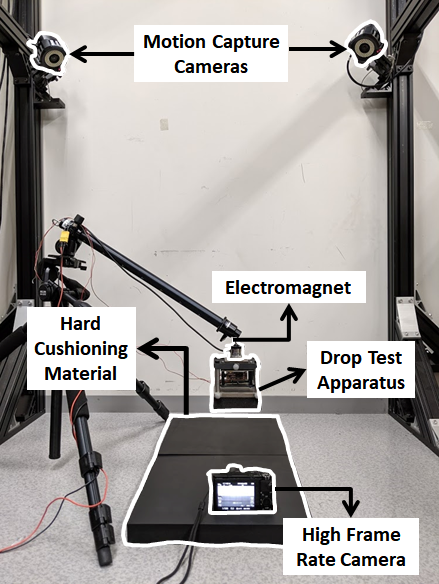
\includegraphics[width=8cm]{./figs/environment.PNG}
        \par\medskip
        Fonte: Própria autoria.
        \label{fig:environment}
\end{figure}

Para cada experimento, o dispositivo é suspenso pelo eletroímã e a altura é medida e ajustada com uma fita-métrica. O goniômetro é utilizado para se certificar que o solo e o corpo de testes estejam paralelos entre si.
Uma vez calibrados, as câmeras, o software de captura de movimento e os sensores são ativados, iniciando a coleta de dados. Após essa etapa, a alimentação do eletroímã é cortada, levando o corpo de prova a uma queda-livre até o impacto ao solo. No final do teste, os dados são reunidos para uma posterior análise.

\section{Simulação do Teste de Queda}

Para a simulação do teste de queda, um programa de \textit{Matlab} foi desenvolvido no ambiente \textit{Simulink}, com o pacote de ferramentas \textit{Simscape Multibody Toolbox}.

O \textit{Simscape Multibody Toolbox} possibilita a simulação 3D de sistemas mecânicos de multicorpos. A construção de modelos é simplificada por meio de diagramas de bloco, os quais podem representar corpos, juntas, forças ou sensores. Outra vantagem é que o \textit{Simscape Multibody Toolbox} formula e resolve as equações de movimento para todo o sistema \cite{simscape}.

No teste de queda, conforme mencionado na seção anterior, uma armação de metal é utilizada para proteger os sensores e fixar o material acolchoado. Um modelo CAD desta armação foi construída em \textit{Solidworks}, mostrado na fig. \ref{fig:corpodeprovacad}, com o objetivo de obter suas características físicas, como matriz de inércia, centro de massa.

 \begin{figure}[H] 
        \centering
        \caption{Armação de metal construído em \textit{Solidworks}.}
        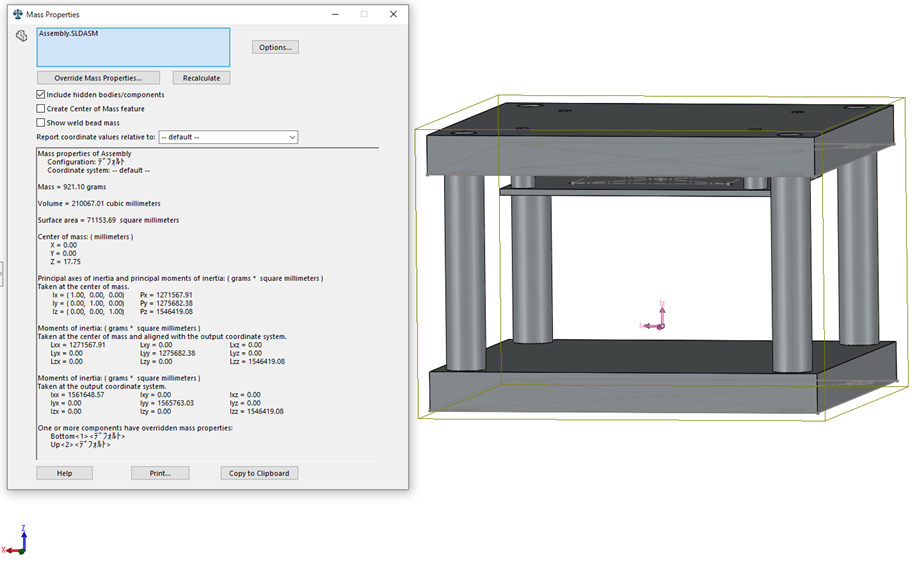
\includegraphics[width=8cm]{./figs/corpodeprova_cad.png}
        \par\medskip
        Fonte: Própria autoria.
        \label{fig:corpodeprovacad}
        %https://learn.sparkfun.com/tutorials/general-guide-to-sparkfun-blocks-for-intel-edison/all
\end{figure}

Essas características físicas são configuradas no modelo simplificado da armação de metal. Nele, sua modelagem é feitos através de um prisma retangular rígido com as mesmas propriedades da peça construída em \textit{Solidworks}. Embora o \textit{Simscape Multibody Toolbox} permita a importação da peça CAD no \textit{Simulink}, seu uso causou instabilidade nas simulações. Desse modo, optou-se em utilizar o modelo simplificado.
O material acolchoado é representado da mesma forma, por um prima retangular, anexado na face inferior da armação de metal, mostrados na fig. \ref{fig:corpodeprovasimulink}, 

 \begin{figure}[H] 
        \centering
        \caption{Ambiente de teste de queda do Simulink, com o corpo de prova. A armação de metal em azul e material acolchoado em cinza}
        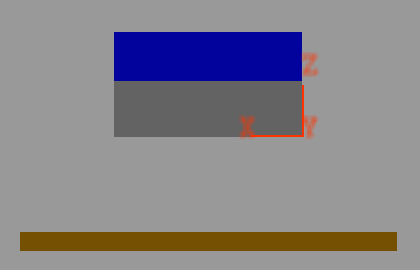
\includegraphics[width=8cm]{./figs/corpodeprova_simulink.png}
        \par\medskip
        Fonte: Própria autoria.
        \label{fig:corpodeprovasimulink}
        %https://learn.sparkfun.com/tutorials/general-guide-to-sparkfun-blocks-for-intel-edison/all
\end{figure}

Vale destacar que no ambiente do \textit{Simulink}, o material acolchoado é tratado como rígido e \textit{Simscape Multibody Toolbox} não calcula as deformações do material, mas a dinâmica do corpo de teste influenciada pela força e torque gerado no impacto com o solo. 
Como será explicado a seguir deste capítulo, uma função a parte será responsável pelo cálculo da deformações do material, e pela força e torque resultantes do impacto ao solo.

Uma das dificuldades da simulação do teste de impacto está na modelagem da força de reação do solo.
Com o material teórico apresentado no capítulo \ref{cap:elementosfinitos}, serão apresentados dois modelos elaborados para essa finalidade. No primeiro modelo, considera-se a força de reação do solo como sendo proporcional ao deslocamento e velocidade dos nós que atravessam o chão. No segundo modelo, considera-se o deslocamento dos nós dentro do solo. 

\subsection{Modelo da Força de Reação do Solo}

Neste modelo, representado na fig. \ref{fig:reactionforcemodel}, o material acolchoado é discretizado por elementos finitos, conforme detalhado no capítulo \ref{cap:elementosfinitos}. Os nós que compõem essa malha são identificados em um de dois grupos. No primeiro estão os nós chamados de fixos, $u_{fix}$, estes nós estão fixados à armação de metal, e assim não possuem deslocamento em relação ao sistema de coordenadas local. Os restantes, chamados de nós livres, $u_{free}$, podem sofrer deformações. 
Para cada nó $j$ da malha, sua posição é dada por:

\begin{equation} \label{eq:position}
    p_{j} = 
    \begin{bmatrix}
        p_{x,j}
        \\
        p_{y,j}
        \\
        p_{z,j}
    \end{bmatrix}
\end{equation}
onde $p_{x,j}, (p_{y,j}, p_{z,j})$ são, respectivamente, as componentes de $p_{j}$ nos eixos $x$, $y$ e $z$.

 \begin{figure}[H] 
        \centering
        \caption{Modelo da Força de Reação do Solo.}
        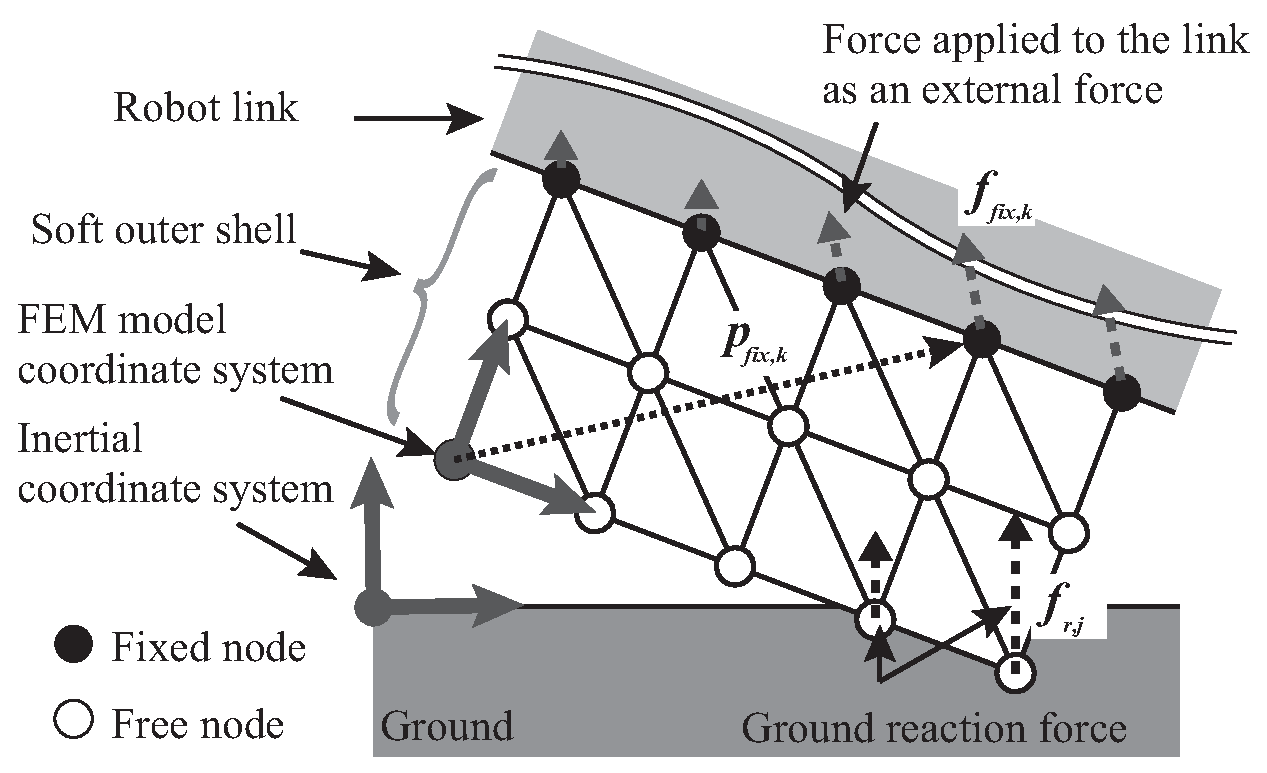
\includegraphics[width=8cm]{./figs/fig2_FEM-MBD_model.eps}
        \par\medskip
        Fonte: 
        \label{fig:reactionforcemodel}
        %https://learn.sparkfun.com/tutorials/general-guide-to-sparkfun-blocks-for-intel-edison/all
\end{figure}

Uma vez identificados, o conjunto $U$ de nós que compõem a malha são reordenados da seguinte maneira:

\begin{equation} \label{eq:fixfreenodes}
    U = 
    \begin{bmatrix}
        u_{free}
        \\
        u_{fix}
    \end{bmatrix}
\end{equation}
onde $u_{free}$ é o conjunto de nós livres e $u_{fix}$ o conjunto de nós fixos.

A força de reação do solo, para o nó $j$ da malha, é definido como \cite{nenchev2018humanoid}:

\begin{equation} \label{eq:floor_force}
        f_{r,j} &= \begin{cases}
    \begin{bmatrix}
        0
        \\
        0
        \\
        -K_{ground}(p_{z,j} - H_{ground}) - D_{ground}\dot{p}_{z,j}
    \end{bmatrix} &\textrm{, se $(p_{z,j} - H_{ground})  < 0$} \\
    
    \begin{bmatrix}
        0
        \\
        0
        \\
        0 
        \end{bmatrix} & \textrm{, caso contrário} \\ 
        \end{cases}
\end{equation}
onde $K_{ground}$ e $K_{ground}$ são, respectivamente, a constante elástica e amortecimento do solo. São parâmetros escolhidos manualmente para a simulação, e possuem os seguintes valores: $K_{ground} = 600$ e $K_{ground} = 0.6$. $(p_{z,j}$ e $\dot{p}_{rz,j}$ são, respectivamente, as componentes no eixo-z da posição e velocidade do nó $j$, escritas no sistema de coordenada global. $H_{ground}$ representa o nível do solo.

Uma vez definido a força $f_{r}$, pode-se escrever a eq. \ref{eq:dynamic} para o conjunto $U$ de nós da malha:

\begin{equation} \label{eq:dynamic}
\pmb{M}\ddot{\pmb{u}} + \pmb{D}\dot{\pmb{u}} + \pmb{K}\pmb{u} = \pmb{f} 
\end{equation}
reordenando os nós conforme \ref{eq:fixfreenodes} e calculando as matrizes $\pmb{M}$, $\pmb{D}$ e $\pmb{K}$, \ref{eq:dynamic} se torna:

\begin{equation} \label{eq:block_dynamic}
     \begin{bmatrix}
            \pmb{M}_0 \quad \pmb{M}_1 \\
            \pmb{M}_2 \quad \pmb{M}_3
    \end{bmatrix}
     \begin{bmatrix}
       \ddot{\pmb{u}}_{free} \\
       \ddot{\pmb{u}}_{fix} 
    \end{bmatrix}    
    + \begin{bmatrix}
            \pmb{D}_0 \quad \pmb{D}_1 \\
            \pmb{D}_2 \quad \pmb{D}_3
         \end{bmatrix}
         \begin{bmatrix}
            \dot{\pmb{u}}_{free} \\
            \dot{\pmb{u}}_{fix} 
         \end{bmatrix}
    + \begin{bmatrix}
            \pmb{K}_0 \quad \pmb{K}_1 \\
            \pmb{K}_2 \quad \pmb{K}_3
         \end{bmatrix}
         \begin{bmatrix}
            \pmb{u}_{free} \\
            \pmb{u}_{fix} 
         \end{bmatrix} =
         \begin{bmatrix}
            \pmb{f}_{free} \\
            \pmb{f}_{fix} 
    \end{bmatrix}
\end{equation}
onde, $u_{fix}$, $\dot{u}_{fix}$ e $\ddot{u}_{fix}$
são, respectivamente, o deslocamento dos nós fixo e suas primeira e segunda derivadas temporais. Como esses nós estão fixos na estrutura, seus valores são nulos. $f_{free}$ é calculado a partir de \ref{eq:floor_force}.
$u_{free}$, $\dot{u}_{free}$, $\ddot{u}_{free}$ e $f_{fix}$ são as incónitas a se determinar.
Da eq. \ref{eq:block_dynamic}, pode-se escrever:

\begin{equation} \label{eq:ufree_calc}
    \pmb{u}_{free} = \pmb{K}_0^{-1}(\pmb{f}_{free} - \pmb{D}_0 \dot{\pmb{u}}_{free} -\pmb{M}_0\ddot{\pmb{u}}_{free})     
\end{equation}
\begin{equation} \label{eq:force_fix_cal}
     \pmb{f}_{fix} = \pmb{K}_2 \pmb{u}_{free} + \pmb{D}_2 \dot{\pmb{u}}_{free} + \pmb{M}_2 \ddot{\pmb{u}}_{free}       
\end{equation}
$u_{free}$, $\dot{u}_{free}$, $\ddot{u}_{free}$ são obtidos resolvendo \ref{eq:ufree_calc} com o método de integração númerica de Newmark, apresentado no capítulo \ref{cap:elementosfinitos}. Uma vez obtidos esses valores, $f_{fix}$ é calculado com a eq. \ref{eq:force_fix_cal}.

Calcula-se o versor de força externa $\mathcal{F}_i$, em relação ao Sistema de Coordenadas Local:

\begin{equation} \label{eq:externalforcetorque}
\pmb{\mathcal{F}}_i
=  \begin{bmatrix}
        \sum_{k=1}^{N_{fix}} \pmb{f}_{fix,k} \\[1em]
        \ \sum_{k=1}^{N_{fix}} \pmb{p}_{fix,k}\times \pmb{f}_{fix,k} \ 
     \end{bmatrix}
\end{equation}
onde $f_{fix}$ é a força aplicada no nó fixo $k$ e $p_{fix}$ é a posição do nó fixo $k$, em relação ao Sistema de Coordenada Local.

Finalmente, os valores de deslocamentos são somados à posição inicial no instante $t$ de cada nó. E essa nova posição é utilizada como posição inicial no seguinte ciclo, $t+1$.

\begin{equation} \label{eq:newposition}
    p^{t+1}_{j} = p^{t}_{j} + u_{j}
\end{equation}


\subsection{Modelo do Deslocamento no Solo}

Neste modelo, representado na fig. \ref{fig:displacementmodel}, o material acolchoado é discretizado por elementos finitos, conforme detalhado no  
capítulo \ref{cap:elementosfinitos}. Os nós que compõem essa malha são identificados em um de dois grupos. No primeiro estão os nós de contato, $U_{con}$. Estes são nós que estão em contato com o solo ou com a armação de metal. Os demais nós, assim como no modelo anterior, são chamados de nós livres, $U_{free}$.
Para cada nó $j$ da malha, sua posição é dada por:

\begin{equation} \label{eq:position}
    p_{j} = 
    \begin{bmatrix}
        p_{x,j}
        \\
        p_{y,j}
        \\
        p_{z,j}
    \end{bmatrix}
\end{equation}
onde $p_{x,j}, (p_{y,j}, p_{z,j})$ são, respectivamente, as componentes de $p_{j}$ nos eixos $x$, $y$ e $z$.

 \begin{figure}[H] 
        \centering
        \caption{Modelo do Deslocamento no Solo.}
        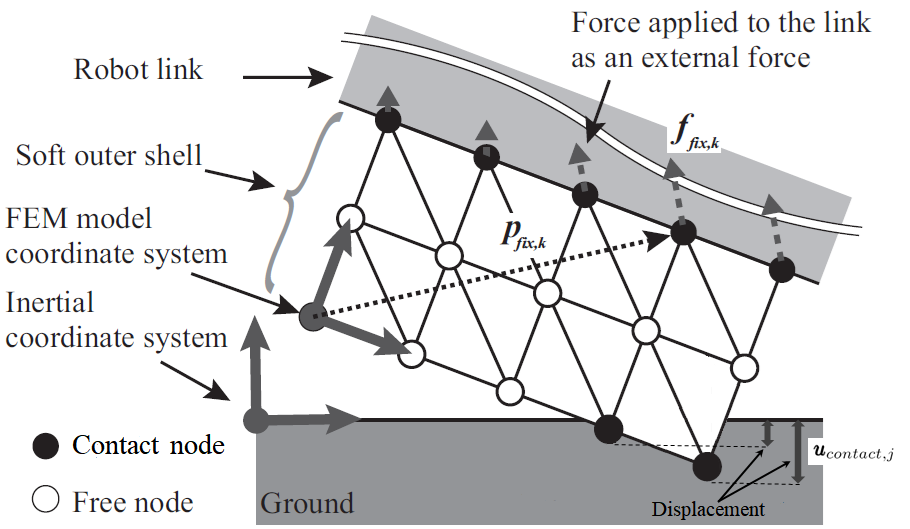
\includegraphics[width=8cm]{./figs/ForcedDisplacementFinal.png}
        \par\medskip
        Fonte: 
        \label{fig:displacementmodel}
        %https://learn.sparkfun.com/tutorials/general-guide-to-sparkfun-blocks-for-intel-edison/all
\end{figure}

Uma vez identificados, o conjunto $U$ de nós que compõem a malha são reordenados da seguinte maneira:

\begin{equation} \label{eq:fixfreenodes}
    U = 
    \begin{bmatrix}
        u_{free}
        \\
        u_{con}
    \end{bmatrix}
\end{equation}
onde $u_{free}$ é o conjunto de nós livres e $u_{con}$ o conjunto de nós de contato.

Ao contrário do modelo anterior, para resolver a eq. \ref{eq:dynamic}, não será calculada a força de reação do solo para cada nó. Ao invés disso, será utilizado o deslocamento dos nós abaixo do solo. Para o nó de contato $j$, seu deslocamento, em relação ao sistema de coordenadas global, é dado por:

\begin{equation} \label{eq:floordisp}
        u^{g}_{con,j} &= \begin{cases}
    \begin{bmatrix}
        0
        \\
        0
        \\
         H_{ground} - {p}_{z,j})
    \end{bmatrix} &\textrm{, se $H_{ground} - {p}_{z,j}) < 0$} \\
    
    \begin{bmatrix}
        0
        \\
        0
        \\
        0 
        \end{bmatrix} & \textrm{, caso contrário} \\ 
        \end{cases}
\end{equation}
onde, $H_{ground}$ e ${p}_{z,j}$ são, respectivamente, o nível do solo e a componente do eixo-$z$ da posição do nó $j$, ambos em relação ao sistema de coordenadas global.

Para expressar o deslocamento em termos do sistema de coordenadas local, uma transformação de coordenadas é aplicado:

\begin{equation} \label{eq:localglobaldisp}
    u_{con, j} = \pmb{R}u^{g}_{con, j} 
\end{equation}

onde $\pmb{R}$ é a matriz de rotação $R$ do sistema de coordenadas global para o sistema de coordenadas local. $u_{con, j}$ é o deslocamento do nó de contato $j$, no sistema de coordenadas local.

Pode-se calcular $\dot{u}_{con}$ e $\ddot{u}_{con}$ da seguinte forma:

\begin{equation}\label{eq:velocdisp}
    \dot{u}_{con} = \frac{{u}_{con}}{\Delta t}
\end{equation}

\begin{equation} \label{eq:accdisp}
        \ddot{u}_{con} = \frac{{\dot{u}}_{con}}{\Delta t}
\end{equation}
onde $\Delta t$ é o intervalo de tempo da simulação.

Reordenando os nós conforme \ref{eq:fixfreenodes} e calculando as matrized $\pmb{M}$, $\pmb{D}$ e $\pmb{K}$, a equação \ref{eq:dynamic} por ser escrita como:

\begin{equation} \label{eq:blockdisp}
 \begin{bmatrix}
        \pmb{M}_0 \quad \pmb{M}_1 \\
        \pmb{M}_2 \quad \pmb{M}_3
\end{bmatrix}
 \begin{bmatrix}
   \ddot{\pmb{u}}_{free} \\
   \ddot{\pmb{u}}_{con} 
\end{bmatrix}    
+ \begin{bmatrix}
        \pmb{D}_0 \quad \pmb{D}_1 \\
        \pmb{D}_2 \quad \pmb{D}_3
     \end{bmatrix}
     \begin{bmatrix}
        \dot{\pmb{u}}_{free} \\
        \dot{\pmb{u}}_{con} 
     \end{bmatrix}
+ \begin{bmatrix}
        \pmb{K}_0 \quad \pmb{K}_1 \\
        \pmb{K}_2 \quad \pmb{K}_3
     \end{bmatrix}
     \begin{bmatrix}
        \pmb{u}_{free} \\
        \pmb{u}_{con} 
     \end{bmatrix} =
     \begin{bmatrix}
        \pmb{f}_{free} \\
        \pmb{f}_{con} 
\end{bmatrix}
\end{equation}
onde $\ddot{u}_{con}$, $\dot{u}_{con}$ e $u_{con}$ são encontrados através das equações \ref{eq:floordisp}, \ref{eq:localglobaldisp}, \ref{eq:velocdisp} e \ref{eq:accdisp}. Além disso $f_{free}$ é um vetor nulo, pois os nós livres não estão sujeitos à força de reação do solo.
Assim $\ddot{u}_{free}$, $\dot{u}_{free}$, $u_{free}$ e $f_{con}$ são as incógnitas a serem calculadas.

Da eq. \ref{eq:blockdisp} pode-se escrever as seguintes equações:

\begin{equation} \label{eq:udispcalc}
    \pmb{M}_0\ddot{\pmb{u}}_{free} +  \pmb{C}_0\dot{\pmb{u}}_{free} +  \pmb{K}_0\pmb{u}_{free} = \pmb{f}_{free} - (\pmb{M}_1\ddot{\pmb{u}}_{con} +  \pmb{C}_1\dot{\pmb{u}}_{con} +  \pmb{K}_1\pmb{u}_{con}) 
\end{equation}

\begin{equation} \label{fdispcalc}
    \pmb{f}_{con} =  \pmb{M}_2\ddot{\pmb{u}}_{free} +  
    \pmb{C}_2\dot{\pmb{u}}_{free} +  \pmb{K}_2\pmb{u}_{free} + 
    \pmb{M}_3\ddot{\pmb{u}}_{con} +  \pmb{C}_3\dot{\pmb{u}}_{con} + \pmb{K}_3\pmb{u}_{con}
\end{equation}
$\ddot{u}_{free}$, $\dot{u}_{free}$ e $u_{free}$ são calculados resolvendo a eq. \ref{eq:udispcalc} através do método de integração numérica apresentado no capítulo \ref{cap:elementosfinitos}. Com estes resultados, encontra-se $f_{con}$ resolvendo a eq. \ref{eq:floordisp}.
 
 A seguir, calcula-se o versor de força externa $\mathcal{F}_i$, em relação ao Sistema de Coordenadas Local:

\begin{equation} \label{eq:externalforcetorque}
\pmb{\mathcal{F}}_i
=  \begin{bmatrix}
        \sum_{k=1}^{N_{con}} \pmb{f}_{con,k} \\[1em]
        \ \sum_{k=1}^{N_{con}} \pmb{p}_{con,k}\times \pmb{f}_{con,k} \ 
     \end{bmatrix}
\end{equation}
onde $f_{con}$ é a força aplicada no nó fixo $k$ e $p_{con}$ é a posição do nó fixo $k$, em relação ao sistema de coordenada local.

Finalmente, os valores de deslocamentos são somados à posição inicial no instante $t$ de cada nó. E essa nova posição é utilizada como posição inicial no seguinte ciclo, $t+1$.

\begin{equation} \label{eq:newposition}
    p^{t+1}_{j} = p^{t}_{j} + u_{j}
\end{equation}

\section{Implementação no Matlab}



\chapter{Resultados e Discussão}\label{cap:resultados}

\lipsum[73]

\section{Base de Dados}

\lipsum[72]

\section{Considerações Finais}

\lipsum[74]

\include{capitulos/conclusao}

% ----------------------------------------------------------
% ELEMENTOS PÓS-TEXTUAIS (Referências, Glossário, Apêndices)
% ----------------------------------------------------------
\postextual

% Referências bibliográficas
\bibliography{bibliografia}

% Glossário (Consulte o manual)
%\glossary

% Apêndices
% ----------------------------------------------------------
% Apêndices
% ----------------------------------------------------------

% ---
% Inicia os apêndices
% ---
\begin{apendicesenv}

% Imprime uma página indicando o início dos apêndices
\partapendices

% ----------------------------------------------------------
\chapter{Primeiro Apêncice}
% ----------------------------------------------------------

\lipsum[50] % Texto qualquer. REMOVER!!

% ----------------------------------------------------------
\chapter{Segundo apêndice com título tão grande quanto se queira porque ele já faz a quebra de linha da coisa toda}
% ----------------------------------------------------------
\lipsum[51-53] % Texto qualquer. REMOVER!!

\end{apendicesenv}
% ---

% Anexos
% ----------------------------------------------------------
% Apêndices
% ----------------------------------------------------------

% ---
% Inicia os anexos
% ---
\begin{anexosenv}

% Imprime uma página indicando o início dos anexos
\partanexos

% ---
\chapter{Nome do Primeiro Anexo}
% ---
\lipsum[30] % Texto qualquer. REMOVER!!

% ---
\chapter{Nome de Outro Anexo}
% ---

\lipsum[32] % Texto qualquer. REMOVER!!

\end{anexosenv}

% Índice remissivo (Consultar manual)
%\phantompart
%\printindex

\end{document}
